%=================================%
\section{Puzzling modal solution}
\label{app:m1q1}
%=================================%

\begin{figure}
	\centering
	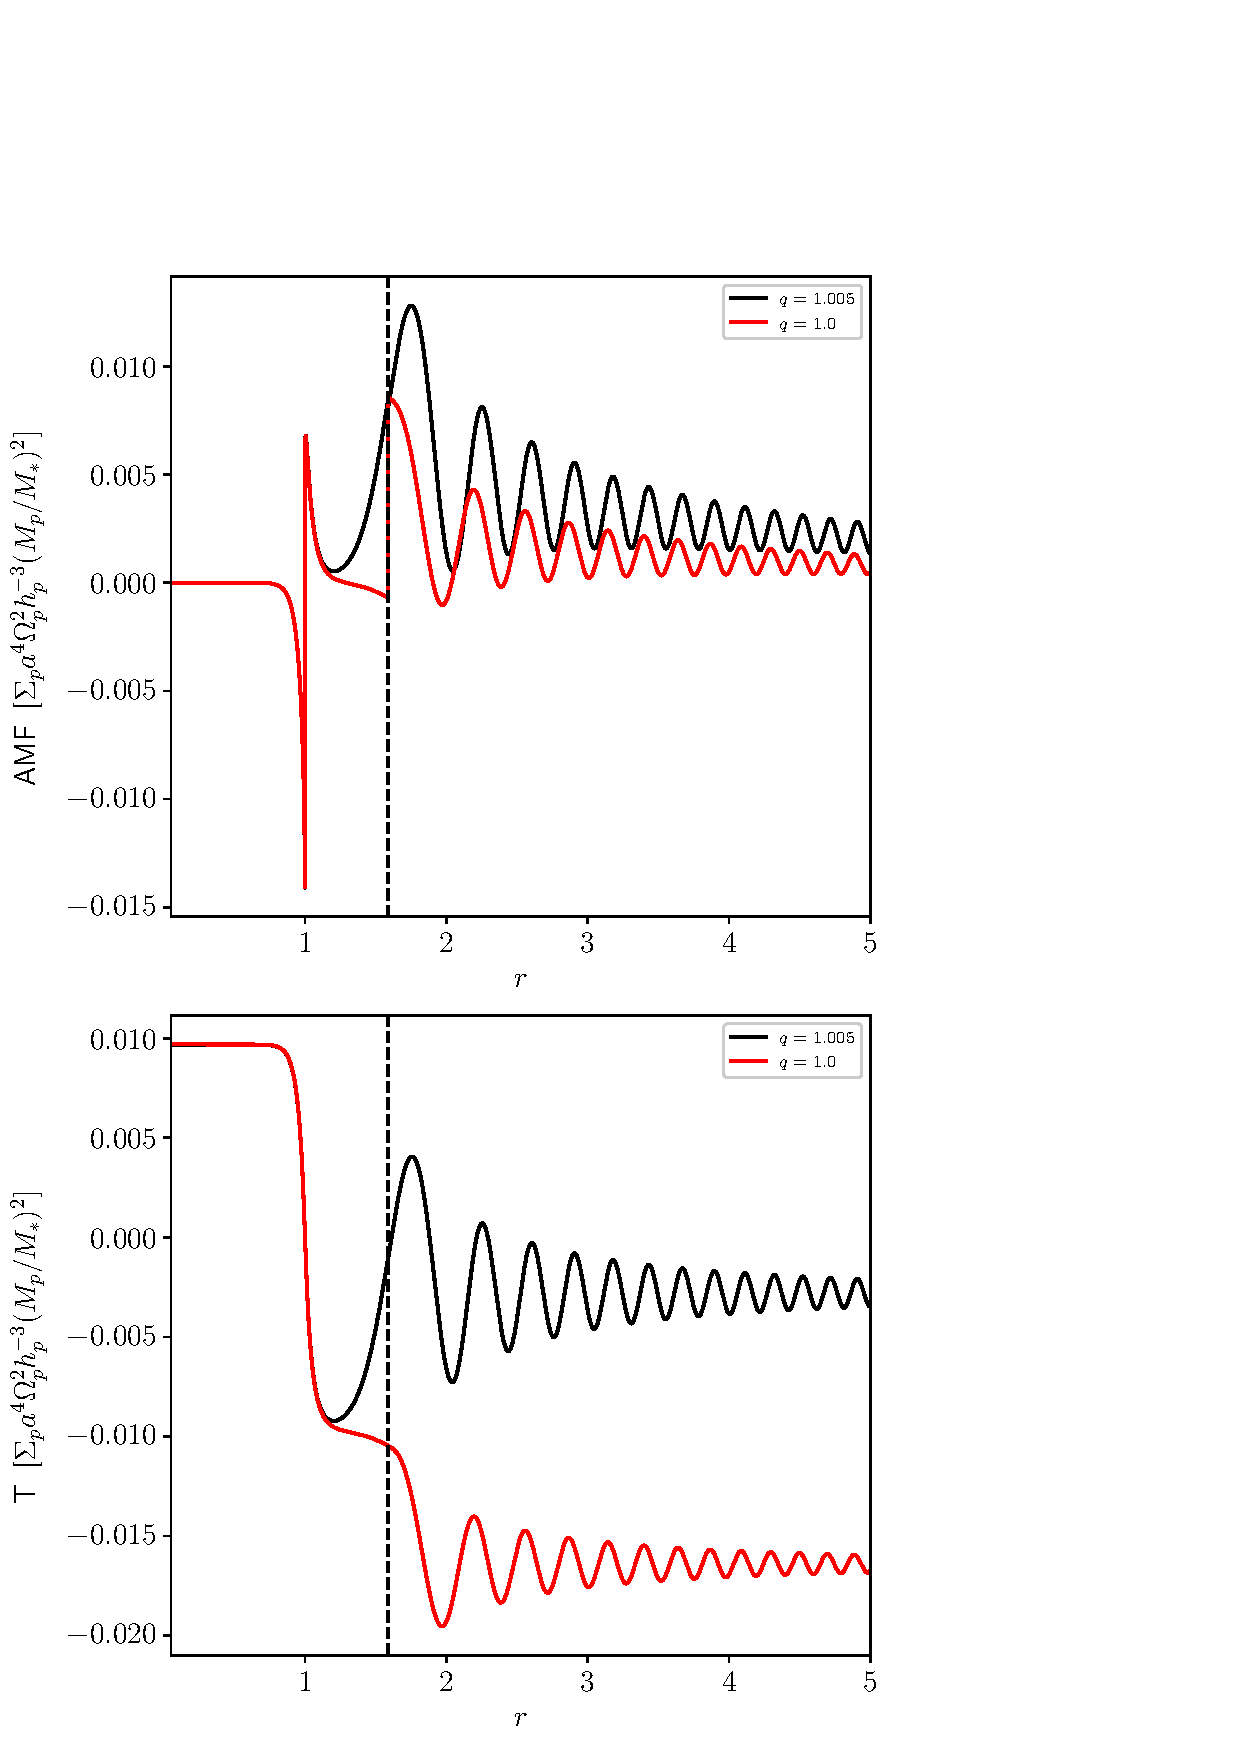
\includegraphics[width=\columnwidth]{Figures/circular_torque_q1.pdf}
	\caption{The $m=1$ response for a disc with $h_\textrm{p} = 0.06$, $b = 0.3$ and $p = 0.0$ for a circular planet with $e = 0.0$. \textit{Upper panel}: angular momentum flux. \textit{Lower panel}: integrated torque. The vertical dashed line shows the position of the outer Lindblad resonance. The red lines correspond to $q=1.0$ whilst the black and green lines (almost overlapping) correspond to $q=1.005$ and $q=0.995$ respectively.}
 \label{fig:circular_q1_torque}
\end{figure}

During the testing of our pipeline for circular orbits with $e = 0.0$, we also extended our runs to larger values of $q$, which highlighted one surprising result. Precisely at the value $q=1.0$ and $p=0.0$ we found that the solution is not well behaved for the $m=1$ mode. In Fig.~\ref{fig:circular_q1_torque} we plot the angular momentum profile for this mode in the upper panel and the integrated radial torque in the lower panel. The red line denotes the special value of $q=1.0$ whilst the black and green lines denote $q=1.005$ and $q=0.995$ respectively. In all cases a uniform surface density is chosen such that $p=0.0$. The dashed grey vertical line denotes the outer Lindblad resonance where there is clearly a discontinuous jump in $F_{J}$ for the $q=1.0$ case, whilst the lines remains smooth for $q = $ 0.995 and 1.005. This spurious behaviour is also echoed in the integrated torque profile which branches off to lower values beyond the outer Lindblad resonance, unlike for values of $q=1.005$ and $q=0.995$ which curve back upwards. By checking a variety of $q$ values approaching 1.0 from above and below we see that this transition in behaviour is sudden and therefore nonphysical. This is seconded by efforts to integrate the equations from a different initial radius which also gave very different looking curves in the case of $q=1.0$, suggesting there is some numerically ill-posed point across the outer Lindblad resonance here. 

Subsequently, when extending our analysis to the full parameter space of eccentric runs, we also noticed some slight deviations in the smooth trends seen in the torque and orbital migration timescale data. This was also traced back to a small handful of spurious $m=1$ modes which present a behaviour similar to that discussed above. Again, this misbehaviour is highly localised in parameter space and slight shifts in the values of $q$ and $p$ characterizing disc properties remove the problem. Throughout this paper we tackle these rare anomalies by actively removing the troublesome modes or infinitesimally shifting the parameter space point to a nearby value. So far we have been unable to track down the origin of this behaviour, which will be deferred for future work.

